%% --- Ensure compat with Acroread -----------------------------------
%%
%% O2 MR for generator upgrades
%%
%%    https://github.com/AliceO2Group/AliceO2/pull/11913
%%
\pdfobjcompresslevel=1
\pdfminorversion=4
% --- Class, packages and theme --------------------------------------
\documentclass[compress,table,8pt]{beamer}
\usetheme[nobuttons,overviews]{alice}
\setbeamertemplate{navigation symbols}{}
\usepackage[export]{adjustbox}%%
\usepackage{multirow}
\usepackage{tikz}
\usetikzlibrary{positioning}
\usetikzlibrary{shapes}
\usetikzlibrary{calc}
\usetikzlibrary{fit}

\newcommand\Rivet{{\scshape Rivet}}
\newcommand\Yoda{{\scshape Yoda}}
\newcommand\HepMC{{\scshape HepMC}}
\newcommand\Otwo{O\textsuperscript{2}}
\newcommand\OtwoPhysics{O\textsuperscript{2}Physics}
\newcommand\AOD{AO\textsuperscript{2}D}
\newcommand\Pythia{{\scshape Pythia}}

%%
%% See https://tex.stackexchange.com/questions/6135/how-to-make-beamer-overlays-with-tikz-node
\tikzset{
  only/.code args={<#1>#2}{%
    \only<#1>{\pgfkeysalso{#2}}
  },
  hide/.style={
    opacity=0,
  },
  show/.style={
    opacity=1
  },
  data/.style={
    shape=ellipse,
    fill=aliceyellow!50!white,
    text=alicegray,
    font=\bfseries\large,
    draw=alicegray
  },
  proc/.style={
    shape=rectangle,
    fill=alicered!50!white,
    text=alicegray,
    font=\bfseries\large,
    draw=alicegray,
  },
  code/.style={
    font=\ttfamily\footnotesize},
  con/.style={
    ->,
    line width=1pt,
    draw=alicegray
  }
}
%% --- Title, and so on ----------------------------------------------
\title{\ALICE{} \Otwo{} and \Rivet}%
\subtitle{\url{https://github.com/cholmcc/O2Physics/tree/cholmcc_pwgmm_rivet/PWGMM/Rivet}\newline%
  {\footnotesize Including this presentation}}
\author[C.H.Christensen]{Christian Holm Christensen}
\institute{\inst{1}Niels Bohr Institute}
\date[12.~Oct, 2023]{12\textsuperscript{th} of October, 2023}
\subject{Rivet}
\titlepageextra{%
  \begin{flushright}
    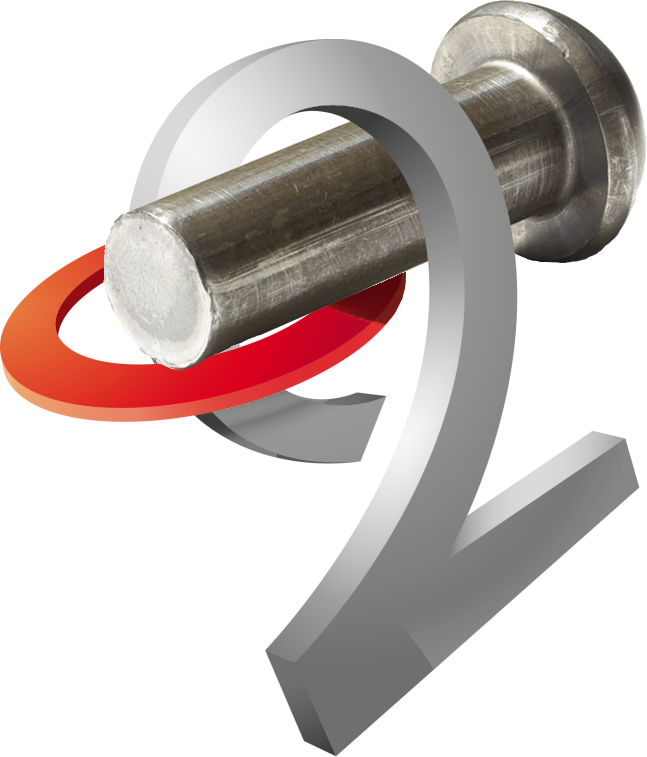
\includegraphics[width=.9\linewidth]{o2rivet}
  \end{flushright}}
\place{PWGMM/MC}
%% === The document ==================================================
\begin{document}
\aliceTitlePage{}
%% ===================================================================
\begin{frame}
  \frametitle{Overview}
  \Overview{}
\end{frame}
%% ===================================================================
\section{Boundary conditions}
\begin{frame}
  \frametitle{The goal of the project}
  \begin{columns}
    \begin{column}{.7\linewidth}
      \begin{itemize}
      \item<+-> Integrate \Rivet{} into the \ALICE{} \Otwo{} pipe-line
        \begin{itemize}
        \item Must work as any other \Otwo{} component
        \end{itemize}
      \item<+-> Leverage existing and future simulation productions
        \begin{itemize}
        \item Read simulation data on disk or on-the-fly
        \end{itemize}
      \item<+-> Lower the threshold for implementation of \ALICE{}
        \Rivet{} analyses
        \begin{itemize}
        \item Large-statistics passes made easy in a familiar fashion
        \end{itemize}
      \end{itemize}
    \end{column}
    \begin{column}{.25\linewidth}
      \begin{tabular}{c}
        
\includegraphics[width=.8\linewidth]{o2}\\
        {\color{gray!75!black}\bfseries\fontsize{48}{0}\selectfont +}\\
        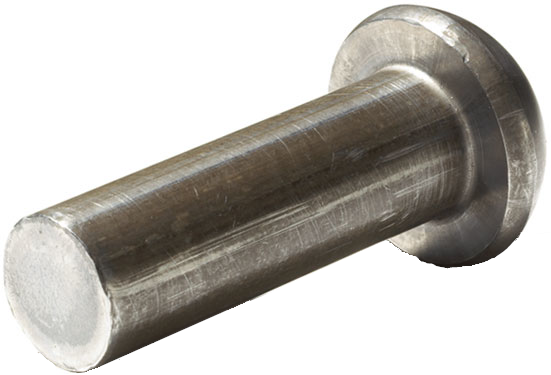
\includegraphics[width=\linewidth]{rivet}
      \end{tabular}
    \end{column}
  \end{columns}
\end{frame}

%% -------------------------------------------------------------------
\begin{frame}
  \frametitle{The steps needed}
  \begin{columns}
    \begin{column}{.6\linewidth}
      \begin{itemize}
      \item<1-> Read in \AOD{}
      \end{itemize}
      \begin{itemize}
      \item<2-> Convert to \HepMC{} event structure
      \end{itemize}
      \begin{itemize}
      \item<3-> Run \Rivet{} on \HepMC{} event structure
      \end{itemize}
      \begin{itemize}
      \item<4-> Store \Yoda{} output
      \end{itemize}
    \end{column}
    \begin{column}{.35\linewidth}
      \begin{center}
        \begin{tikzpicture}
          \node[data,hide,only={<1->{show}}] (aod) {\AOD};
          \node[proc,hide,only={<2->{show}},below=6mm of aod.south] (cnv) {Convert};
          \node[data,hide,only={<2->{show}},below=6mm of cnv.south] (evt) {\HepMC};
          \node[proc,hide,only={<3->{show}},below=6mm of evt.south] (rvt) {\Rivet};
          \node[data,hide,only={<4->{show}},below=6mm of rvt.south] (yda) {\Yoda};
          \draw[con,hide,only={<2->{show}}] (aod)--(cnv);
          \draw[con,hide,only={<2->{show}}] (cnv)--(evt);
          \draw[con,hide,only={<3->{show}}] (evt)--(rvt);
          \draw[con,hide,only={<4->{show}}] (rvt)--(yda);
        \end{tikzpicture}
      \end{center}
    \end{column}
  \end{columns}
\end{frame}

%% -------------------------------------------------------------------
\begin{frame}
  \frametitle{With a bit more details}
  \begin{itemize}
  \item<+-> Convert \AOD{} simulation data to to \HepMC{} event structure
    \begin{itemize}
    \item \texttt{MCParticles} to \texttt{HepMC3::GenParticle} and
      \texttt{HepMC3::Vertex}
    \item \texttt{MCCollisions} to event number, and weight
    \item Also auxiliary information
      \begin{itemize}
      \item \texttt{HepMCXSections} to \texttt{HepMC3::CrossSection}
        --- $\sigma$ and $\delta\sigma$, possibly multiple
      \item \texttt{HepMCPdfInfos} to \texttt{HepMC3::PdfInfo} ---
        parton distribution parameters
      \item \texttt{HepMCHeavyIons} to \texttt{HepMC3::HeavyIon} ---
        event ``geometry'' parameters $N_{\mathrm{coll}}$,
        $N_{\mathrm{part}}$, etc.
      \item Relevant \Otwo{} commits: MR
        \href{https://github.com/AliceO2Group/AliceO2/pull/12032/commits}{\#
          12032} and
        \href{https://github.com/AliceO2Group/AliceO2/commit/d3bcb9d5c98a14618e100c4d476103b8f5989ae1}{d3bcb9d}
      \end{itemize}
    \end{itemize}
  \item<+-> Pass \texttt{HepMC3::GenEvent} to \Rivet{} Manager
  \item<+-> Let \Rivet{} manager run analyses over data
    \begin{itemize}
    \item Select analyses
    \item Set load path for compile code and data
    \item Compile analysis code and load it
    \item Load auxiliary data --- e.g., for centrality calibrations
    \end{itemize}
  \item<+-> Store results of \Rivet{} analyses (\Yoda{} Analysis Objects
    --- AOs) in output file
  \item<+-> Run analyses \texttt{finalize} method on AOs
    \begin{itemize}
    \item Including cases where the AOs where merged from multiple
      jobs --- e.g., Grid execution
    \item To be done ``by-hand'' by user.
    \end{itemize}
  \end{itemize}
\end{frame}

%% ===================================================================
\section{\HepMC{} events}
\begin{frame}
  \frametitle{A \HepMC{} event}
  \begin{center}
    \includegraphics[width=.8\linewidth]{%
      crmc_eposlhc_119052862_p_p_3500_event000000.gv.pdf}
  \end{center}
  EPOS-LHC pp at $\sqrt{s}=\TeV[7]$

  {\footnotesize Visualised by \texttt{Tools/hepmc.py} in
    \href{https://github.com/cholmcc/O2Physics/tree/cholmcc_pwgmm_rivet/PWGMM/Rivet}{project}.}
\end{frame}

\begin{frame}
  \frametitle{Transport of an event}
  \begin{columns}[t,onlytextwidth]
    \begin{column}{.2\linewidth}
      \begin{block}{Before}
        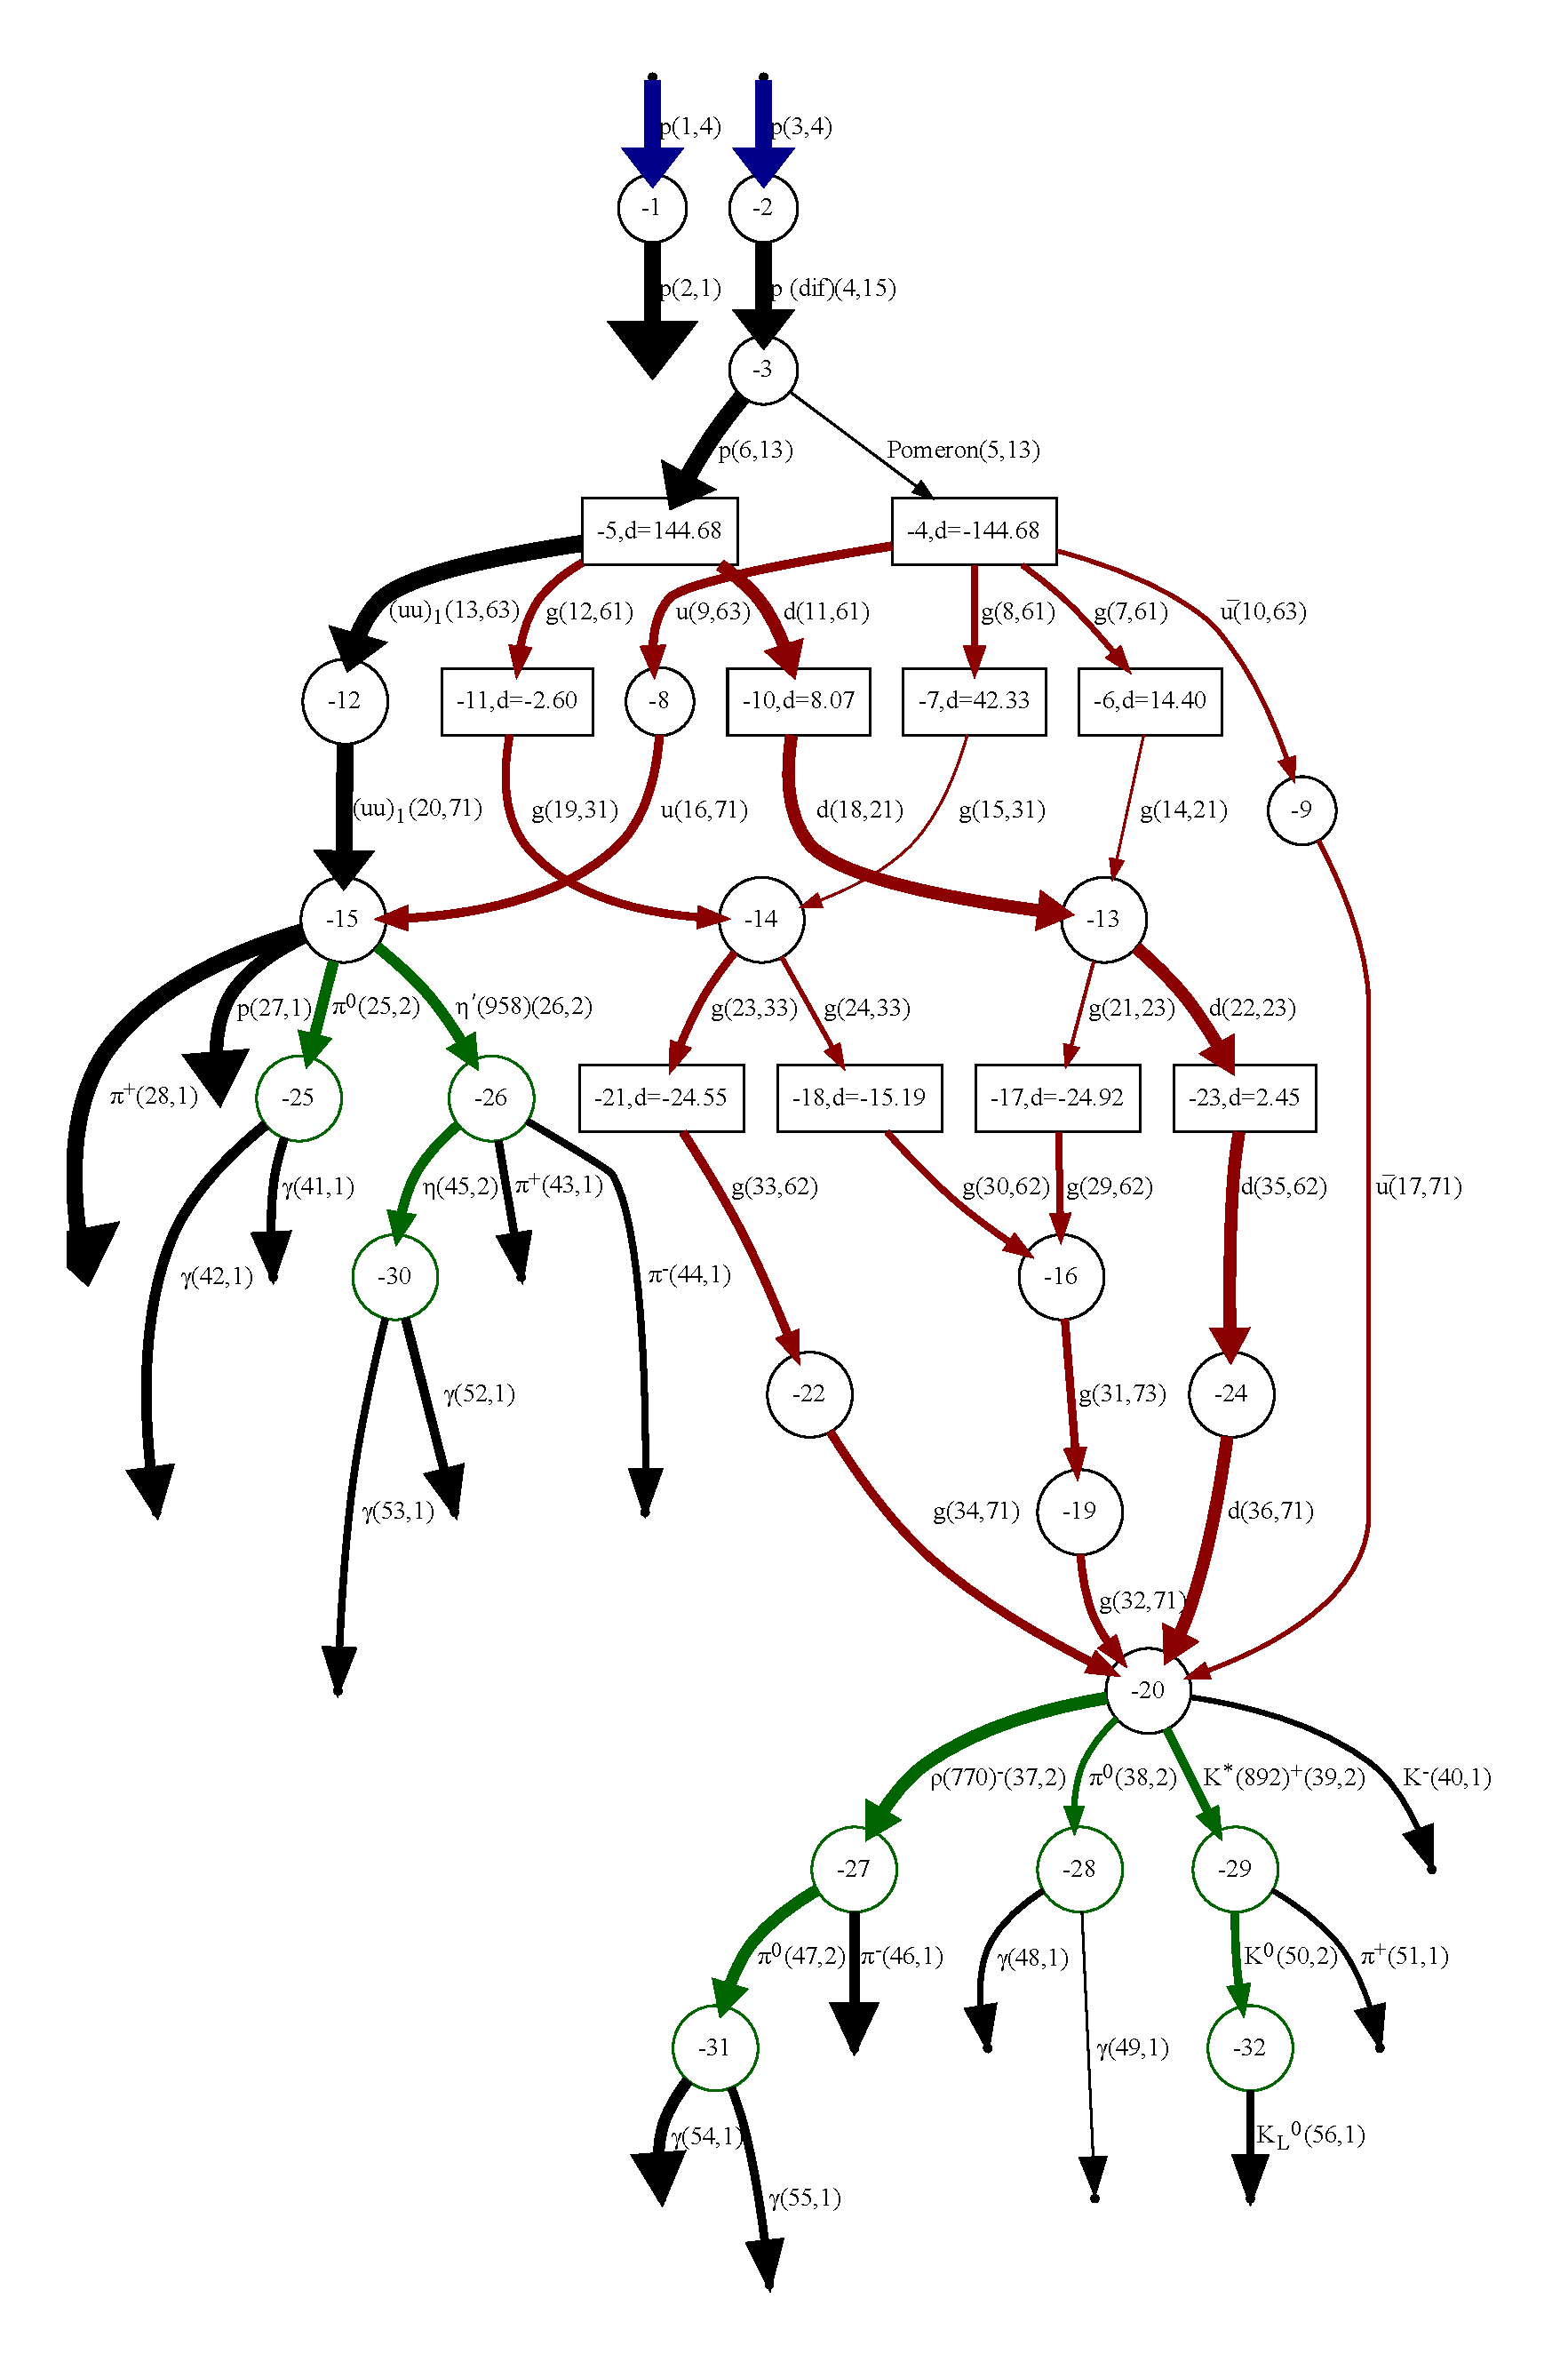
\includegraphics[width=\linewidth]{genpythia_event000000.gv.pdf}
      \end{block}
    \end{column}
    \begin{column}<2->{.75\linewidth}
      \begin{block}{After}
        \includegraphics[width=\linewidth]{genpythia_Kine_event000000.gv.pdf}
      \end{block}
    \end{column}
  \end{columns}
  \Pythia{} pp at $\sqrt{s}=\TeV[14]$, a single-diffractive event

  {\footnotesize(Anything else would be even more illegible)}
\end{frame}

%% -------------------------------------------------------------------
\begin{frame}
  \frametitle{\AOD{} $\rightarrow$ \HepMC{} Event}

  \begin{columns}[onlytextwidth,t]
    \begin{column}{.4\linewidth}
      \begin{itemize}
      \item<+-> Done by ``helper'' class
        \texttt{o2::eventgen::AODToHepMC} in
        \href{https://github.com/AliceO2Group/AliceO2/blob/dev/Generators/include/Generators/AODToHepMC.h}{\texttt{AODToHepMC.h}}
        and
        \href{https://github.com/AliceO2Group/AliceO2/blob/dev/Generators/src/AODToHepMC.cxx}{\texttt{AODToHepMC.cxx}}
        \newline%
        {\footnotesize Relevant \Otwo{} commits:
          \href{https://github.com/AliceO2Group/AliceO2/pull/12038/commits}{MR
            \# 12038}}
      \item<+-> Reads in \AOD{} tables
        \begin{itemize}
        \item \texttt{MCParticles}
        \item \texttt{MCCollisions}
        \item \texttt{HepMCXSections}
        \item \texttt{HepMCPdfInfos}
        \item \texttt{HepMCHeavyIons}
        \end{itemize}
      \item<+-> Generates
        \begin{itemize}
        \item \texttt{HepMC3::GenEvent}
        \item \texttt{HepMC3::GenVertex} \& \texttt{HepMC3::GenParticle}
        \item \texttt{HepMC3::GenCrossSection}
        \item \texttt{HepMC3::GenPdfInfo}
        \item \texttt{HepMC3::GenHeavyIon}
        \end{itemize}
      \item<+-> \texttt{HepMC3::GenEvent} kept in-memory.
      \end{itemize}
    \end{column}
    \begin{column}{.55\linewidth}
      \begin{center}
        \begin{tikzpicture}
          \begin{scope}[hide,only={<2->{show}}]
            \node[] (aodt) {\AOD{}};
            \node[data,code,below=3mm of aodt.south] (mcpart) {%
              \texttt{MCParticles}};
            \node[data,code,below=2mm of mcpart.south] (mccoll) {%
              \texttt{MCCollisions}};%
            \node[data,code,below=2mm of mccoll.south] (mcxsec) {%
              \texttt{HepMCXSections}};%
            \node[data,code,below=2mm of mcxsec.south] (mcpdfs) {%
              \texttt{HepMCPdfInfos}};
            \node[data,code,below=2mm of mcpdfs.south] (mchvyi) {%
              \texttt{HepMCHeavyIons}};
            \node[draw=alicegray,
            fit={(aodt)(mcpart)(mccoll)(mcxsec)(mcpdfs)(mchvyi)}]{};
          \end{scope}
          \begin{scope}[hide,only={<3->{show}}]
            \node[right=2cm of aodt.east,code] (hept) {\texttt{GenEvent}};
            \node[data,code,below=3mm of hept.south] (part) {%
              \texttt{GenParticle}};
            \node[data,code,below=2mm of part.south] (vrtx) {%
              \texttt{GenVertex}};%
            \node[data,code,below=2mm of vrtx.south] (xsec) {%
              \texttt{GenCrossSection}};%
            \node[data,code,below=2mm of xsec.south] (pdfi) {%
              \texttt{GenPdfInfo}};
            \node[data,code,below=2mm of pdfi.south] (hvyi) {%
              \texttt{GenHeavyIon}};
            \node[draw=alicegray,
            fit={(hept)(part)(vrtx)(xsec)(pdfi)(hvyi)}] (hep) {};
          \end{scope}
          \draw[con,hide,only={<3->{show}}] (mcpart)--(part);
          \draw[con,hide,only={<3->{show}}] (mcpart)--(vrtx);
          \draw[con,hide,only={<3->{show}}] (mcxsec)--(xsec);
          \draw[con,hide,only={<3->{show}}] (mcpdfs)--(pdfi);
          \draw[con,hide,only={<3->{show}}] (mchvyi)--(hvyi);
          \draw[con,hide,only={<3->{show}}] (mccoll)--(hep);
        \end{tikzpicture}
      \end{center}
      \vspace*{1ex} \uncover<3->{
        %% Linter wants space before parenthesis - may be entirely
        %% wrong here.
        Recent upgrade to \Otwo{} fixes all paths for ``official''
        productions.}
    \end{column}
  \end{columns}
\end{frame}

%% ===================================================================
\section{\Rivet{} run}
%% -------------------------------------------------------------------
\begin{frame}
  \frametitle{\HepMC{} $\rightarrow$ \Rivet{}}

  \begin{columns}[onlytextwidth]
    \begin{column}{.6\linewidth}
      \begin{itemize}
      \item<+-> Done by ``helper'' class \texttt{o2::rivet::Wrapper}
        in
        \href{https://https://github.com/cholmcc/O2Physics/tree/cholmcc_pwgmm_rivet/PWGMM/Rivet/Tasks/Wrapper.h}{\texttt{O2RivetWrapper.h}}
      \item<+-> Holds a \texttt{Rivet::AnalysisHandler} object
      \item<+-> Get in-memory \texttt{HepMC3::GenEvent} (from
        \texttt{AODToHepMC}).
      \item<+-> Executes registered analyses passing event to
        \texttt{Rivet::Analysis::event}
      \item<+-> At end of job, stores \Yoda{} AOs in
        \texttt{o2::rivet::RivetAOs}
        (\href{https://https://github.com/cholmcc/O2Physics/tree/cholmcc_pwgmm_rivet/PWGMM/Rivet/DataModel/RivetAOs.h}{\texttt{RivetAOs.h}})
        object written to \texttt{AnalysisResults.root} file.
        \begin{itemize}
        \item<+-> This uses a hack by registering a
          \texttt{OutputManager<o2::rivet::Wrapper>} in workflow.
        \item<+-> Documentation advertises an \texttt{endRun} call-back,
          but that is never called!
        \item<+-> I miss \texttt{AliAnalysisTask::LocalTerminate} and
          \texttt{AliAnalysisTask::Terminate}.
        \end{itemize}
      \end{itemize}
    \end{column}
    \begin{column}{.35\linewidth}
      \begin{center}
        \begin{tikzpicture}
          \node[data,hide,only={<3->{show}}] (evt) {\texttt{HepMC::GenEvent}};
          \node[proc,hide,text width=7em,align=center,only={<1->{show}},below=6mm of evt.south] (wrp) {%
            \texttt{Wrapper}\newline
            {\footnotesize\texttt{AnalysisHandler}}
          };
          \node[proc,hide,text width=7em,align=center,only={<4->{show}},below=6mm of wrp.south] (ana) {
            \texttt{Analysis}\newline
            {\footnotesize one or more}};
          \node[data,hide,only={<5->{show}},below=6mm of ana.south] (out) {%
            \texttt{Output}};
          \draw[con,hide,only={<3->{show}}] (evt)--(wrp);
          \draw[con,hide,only={<4->{show}}] (wrp)--(ana);
          \draw[con,hide,only={<5->{show}}] (ana)--(out);
        \end{tikzpicture}
      \end{center}
    \end{column}
  \end{columns}

\end{frame}

%% -------------------------------------------------------------------
\begin{frame}
  \frametitle{\Rivet{} wrapper}

  ``Helper'' class \texttt{o2::rivet::Wrapper} in
  \href{https://https://github.com/cholmcc/O2Physics/tree/cholmcc_pwgmm_rivet/PWGMM/Rivet/Tasks/Wrapper.h}{\texttt{Wrapper.h}}

  \begin{columns}[onlytextwidth,t]
    \begin{column}{.45\linewidth}
      \begin{itemize}
      \item<+-> List of analysis to execute
      \item<+-> Load paths of analyses and data
      \item<+-> Data to pre-load\newline {\footnotesize E.g.,
          centrality calibrations}
      \item<+-> Can compile source files to shared library \newline
        {\footnotesize E.g., upload analysis source and build in
          target environment}
      \item<+-> \textellipsis{} and more
      \end{itemize}
    \end{column}
    \begin{column}{.45\linewidth}
      \begin{itemize}
      \item<1-> \texttt{--rivet-analyses}
      \item<2-> \texttt{--rivet-load-paths}
      \item<3-> \texttt{--rivet-pre-loads}
      \item<4-> \texttt{--rivet-sources}
      \item<5-> \texttt{--rivet-flags} for compiler/linker
      \item<5-> \texttt{--rivet-pwd} for loader
      \item<5-> \texttt{--rivet-ignore-beams}
      \item<5-> \texttt{--rivet-cross-section} override \HepMC{}
      \item<5-> \texttt{--rivet-finalize}
      \item<5-> \texttt{--rivet-log} for \Rivet{} logging
      \end{itemize}
    \end{column}
  \end{columns}
\end{frame}

%% ===================================================================
\section{Output object}
\begin{frame}
  \frametitle{\Rivet{} results}
  \begin{itemize}
  \item<+-> \texttt{o2::rivet::RivetAOs}
    (\href{https://https://github.com/cholmcc/O2Physics/tree/cholmcc_pwgmm_rivet/PWGMM/Rivet/Tasks/Wrapper.h}{\texttt{RivetAOs.h}})
    \begin{itemize}
    \item<+-> Contains \Yoda{} AOs streamed to a string
    \item<+-> Stores load paths, needed by merge\newline%
      {\footnotesize perhaps also store compiled sources?}
    \item<+-> Can be merged as
      \texttt{o2::mergers::MergeInterface} or \texttt{TObject::Merge}.
      \begin{itemize}
      \item<+-> According Anton Alkin, no user workflow code called
        when merging \texttt{AnalysisResults.root}\newline%
        {\footnotesize \texttt{AliAnalysisTask::Terminate} is gone}
      \item<+-> \texttt{AliPhysics}$\rightarrow$\Otwo{} regression!
      \end{itemize}
    \item<+-> Easily saved to \Yoda{} file (\emph{script}
      \texttt{WriteOutput.C}).
    \end{itemize}
  \end{itemize}
\end{frame}

%% ===================================================================
\section{Workflow}
\begin{frame}[fragile]
  \frametitle{Workflow}

  \begin{itemize}
  \item<+-> \texttt{o2-analysis-mm-rivet} in
    (\href{https://github.com/cholmcc/O2Physics/tree/cholmcc_pwgmm_rivet/PWGMM/Rivet/Tasks/rivet.cxx}{\texttt{rivet.cxx}})
  \item<+-> Uses objects of ``helper'' classes
    \texttt{o2::eventgen::AODToHepMC} and \texttt{o2::rivet::Wrapper}.
  \item<+-> By default reads \AOD{} \texttt{MCCollisions}
    and \texttt{MCParticles}\newline
    {\footnotesize Relevant \Otwo{} commits:
      \href{https://github.com/AliceO2Group/AliceO2/pull/12032/commits}{MR
        \# 12032}
      and
      \href{https://github.com/AliceO2Group/AliceO2/commit/d3bcb9d5c98a14618e100c4d476103b8f5989ae1}{d3bcb9d}
    }
  \item<+-> \emph{Can} also read in auxiliary \AOD{} tables\newline
    {\footnotesize Had problems with \texttt{PROCESS\_SWITCH} --- To
      be investigated}
  \end{itemize}

  \setbeamercolor{block body example}{bg=gray!25!white}
  \begin{exampleblock}<+->{Example}
\begin{verbatim}
o2-analysis-mm-rivet --aod-file AO2D.root --rivet-pwd \
  --rivet-analysis ALICE_YYYY_I1234567 \
  --rivet-sources ALICE_YYYY_I1234567.C
\end{verbatim}
  \end{exampleblock}
  \uncover<+->{Note, \OtwoPhysics{} code-checker doesn't like standard
    ending \texttt{.cc}}
\end{frame}

%% -------------------------------------------------------------------
\begin{frame}[fragile]
  \frametitle{Longer examples}
  \setbeamercolor{block body example}{bg=gray!25!white}
  \begin{exampleblock}<+->{With production}
\begin{verbatim}
o2-sim -n 100 -g pythia8pp -o pythia8pp
o2-aod-mc-producer-workflow  --mckine-fname pythia8pp | \
  o2-analysis-mm-rivet --rivet-pwd \
    --rivet-analysis ALICE_YYYY_I1234567 \
    --rivet-sources ALICE_YYYY_I1234567.C
\end{verbatim}
  \end{exampleblock}

  \begin{exampleblock}<+->{As service}
\begin{verbatim}
o2-sim -n 100 -g pythia8pp -o pythia8pp --forward-kine --noDiscOutput &
o2-kine-publisher --nevents 100 --o2sim-pid $! --aggregate-timeframe 1 | \
  o2-sim-mctracks-to-aod | \
  o2-analysis-mm-rivet --rivet-pwd \
    --rivet-analysis ALICE_YYYY_I1234567 \
    --rivet-sources ALICE_YYYY_I1234567.C
\end{verbatim}
  \end{exampleblock}
  \uncover<2->{
    {\footnotesize{} (BTW, it should be
      \texttt{--noDis{\itshape{}k\/}Output}), see
      \href{https://www.grammarly.com/blog/disc-disk/}{here} --- So much
      AliNglish.}}
\end{frame}

%% -------------------------------------------------------------------
\begin{frame}[fragile]
  \frametitle{Merge and finalize}

  \setbeamercolor{block body example}{bg=gray!25!white}
  \begin{exampleblock}<+->{Two \AOD{}s}
\begin{verbatim}
o2-analysis-mm-rivet --aod-file AO2D_1.root --rivet-pwd \
  --rivet-analysis ALICE_YYYY_I1234567 \
  --rivet-sources ALICE_YYYY_I1234567.C && \
  mv AnalysisResults.root AnalysisResults_1.root
o2-analysis-mm-rivet --aod-file AO2D_2.root --rivet-pwd \
  --rivet-analysis ALICE_YYYY_I1234567 \
  --rivet-sources ALICE_YYYY_I1234567.C && \
  mv AnalysisResults.root AnalysisResults_2.root
hadd finalized.root AnalysisResults_1.root AnalysisResults_2.root
root -l -b -q WriteOutput\(\"finalized.root\"\)
ipython3 -i ALICE_YYYY_I1234567.py finalized.yoda
\end{verbatim}
  \end{exampleblock}

  \uncover<+->{\alert{Includes} \texttt{Rivet::Analysis::finalize}}
\end{frame}

%% ===================================================================
\section{Summary}
\begin{frame}
  \frametitle{Where are we now?}

  \begin{columns}[onlytextwidth,t]
    \begin{column}{.45\linewidth}
      \begin{block}{Status}
        \begin{itemize}
        \item<+-> \AOD{} to \HepMC{} done
        \item<+-> \Rivet{} wrapper on \HepMC{} from \AOD{} done\newline%
          {\footnotesize \texttt{\OtwoPhysics{} merge request
            \href{https://github.com/AliceO2Group/O2Physics/pull/4400}{4400}}}
          \begin{itemize}
          \item Specify analyses
          \item Specify load paths
          \item Specify pre-loaded data
          \item Output stored in
            \texttt{AnalysisResults.root}
          \item Merges as \texttt{TObject}\newline%
            {\footnotesize including
              \texttt{Rivet::Analysis::finalize}}
          \end{itemize}
        \item<+-> \HepMC{} aux to \texttt{MCEventHeader} done
        \item<+-> \HepMC{} aux to \AOD{} done
        \item<+-> Update and deploy \Rivet{} in environments
          \begin{itemize}
          \item \texttt{alidist} merge request
            \href{https://github.com/alisw/alidist/pull/5320}{5320}
            for CVMFS
          \end{itemize}
        \end{itemize}
      \end{block}
    \end{column}
    \begin{column}{.45\linewidth}
      \begin{alertblock}{Open}
        \begin{itemize}
        \item<+-> Deploy on HyperLoop.
        \end{itemize}
      \end{alertblock}
      \begin{center}
        \includegraphics<+->[width=.5\linewidth]{o2rivet}
      \end{center}
    \end{column}
  \end{columns}
\end{frame}


%% ===================================================================
\begin{frame}
  \vfill
  {\Huge Backups}\\[2ex]
  % {but may add diagram for talks, preliminaries, etc}
  \vfill
\end{frame}

%% -------------------------------------------------------------------
\begin{frame}
  \frametitle{HepMC auxiliary to \texttt{MCEventHeader}}

  {Commits of merge request \alert{\href{https://github.com/AliceO2Group/AliceO2/pull/12032/commits}{\# 12032}}}

  \begin{itemize}[<+->]
  \item \texttt{GeneratorPythia8} fill in available HepMC aux\newline
    {\footnotesize Uses different info than \Pythia{} authors use for
      f.ex.~$N_{\mathrm{coll}}$}
  \item \texttt{GeneratorHepMC} fill in all available in input
    \begin{itemize}
    \item Also support execute EG in background and stream HepMC event
      to FIFO\newline
      (Almost) \emph{Any} HepMC EG supported via this.
    \end{itemize}
  \item Predefined \texttt{o2::dataformats::MCEventHeader} key strings
    (\texttt{o2::dataformats::MCInfoKeys}).
  \end{itemize}

\end{frame}

%% -------------------------------------------------------------------
\begin{frame}
  \frametitle{HepMC auxiliary to \AOD{}}

  {Commit
    \alert{\href{https://github.com/AliceO2Group/AliceO2/commit/d3bcb9d5c98a14618e100c4d476103b8f5989ae1}{d3bcb9d}}}:

  \begin{itemize}[<+->]
  \item Refactor \texttt{o2-aod-mc-producer-workflow},
    \texttt{o2-aod-producer-workflow}, and \texttt{o2-sim-kine-to-aod}
    to common \texttt{o2::aodmchelper} functions.
  \end{itemize}

\end{frame}

\end{document}
%% Local Variables:
%%   ispell-dictionary: "british"
%%   mode: LaTeX
%% End:
%%
%% EOF
%%

%  LocalWords:  Parameterisation parameterisation
